\emph{Elektromagnetisk vågutbredning är energitransport och
  förutsättningen för all radiokommunikation. Radiovågornas utbredning
  på vägen mellan sändare och mottagare påverkas emellertid på många
  sätt. Med vetskap om radiovågornas utbredningssätt kan man mer
  metodiskt försöka uppnå önskade radioförbindelser.}

\section[Kraftfält antenner]{Kraftfälten omkring antenner}

För att sända ut och ta emot radiovågor behövs antenner. Mycket
förenklat är en antenn en elektrisk krets, som består av en induktor
och en kondensator.

Med kondensatorns elektroder helt isärdragna och förminskade har
svängningskretsen fått ett mycket annorlunda mekaniskt utseende. Sedan
induktorn i LC-kretsen tagits bort, så återstår mekaniskt sett endast
en enkel ledare, men elektriskt sett finns kretsen ändå kvar. Ledaren
med sin utsträckning är fortfarande en induktor och ytorna på dess
motstående halvor är fortfarande elektroderna i kondensatorn med
omgivningen som dielektrikum.

En elektrisk ledare, en stång, tråd etc. är alltså en elektrisk
svängningskrets, vars resonansfrekvens mest bestäms av längden och
tjockleken. Ledaren (antennen) kan kallas dipol -- den har två
poler. Se bild \ref{fig:BildII7-01}.

\begin{figure}
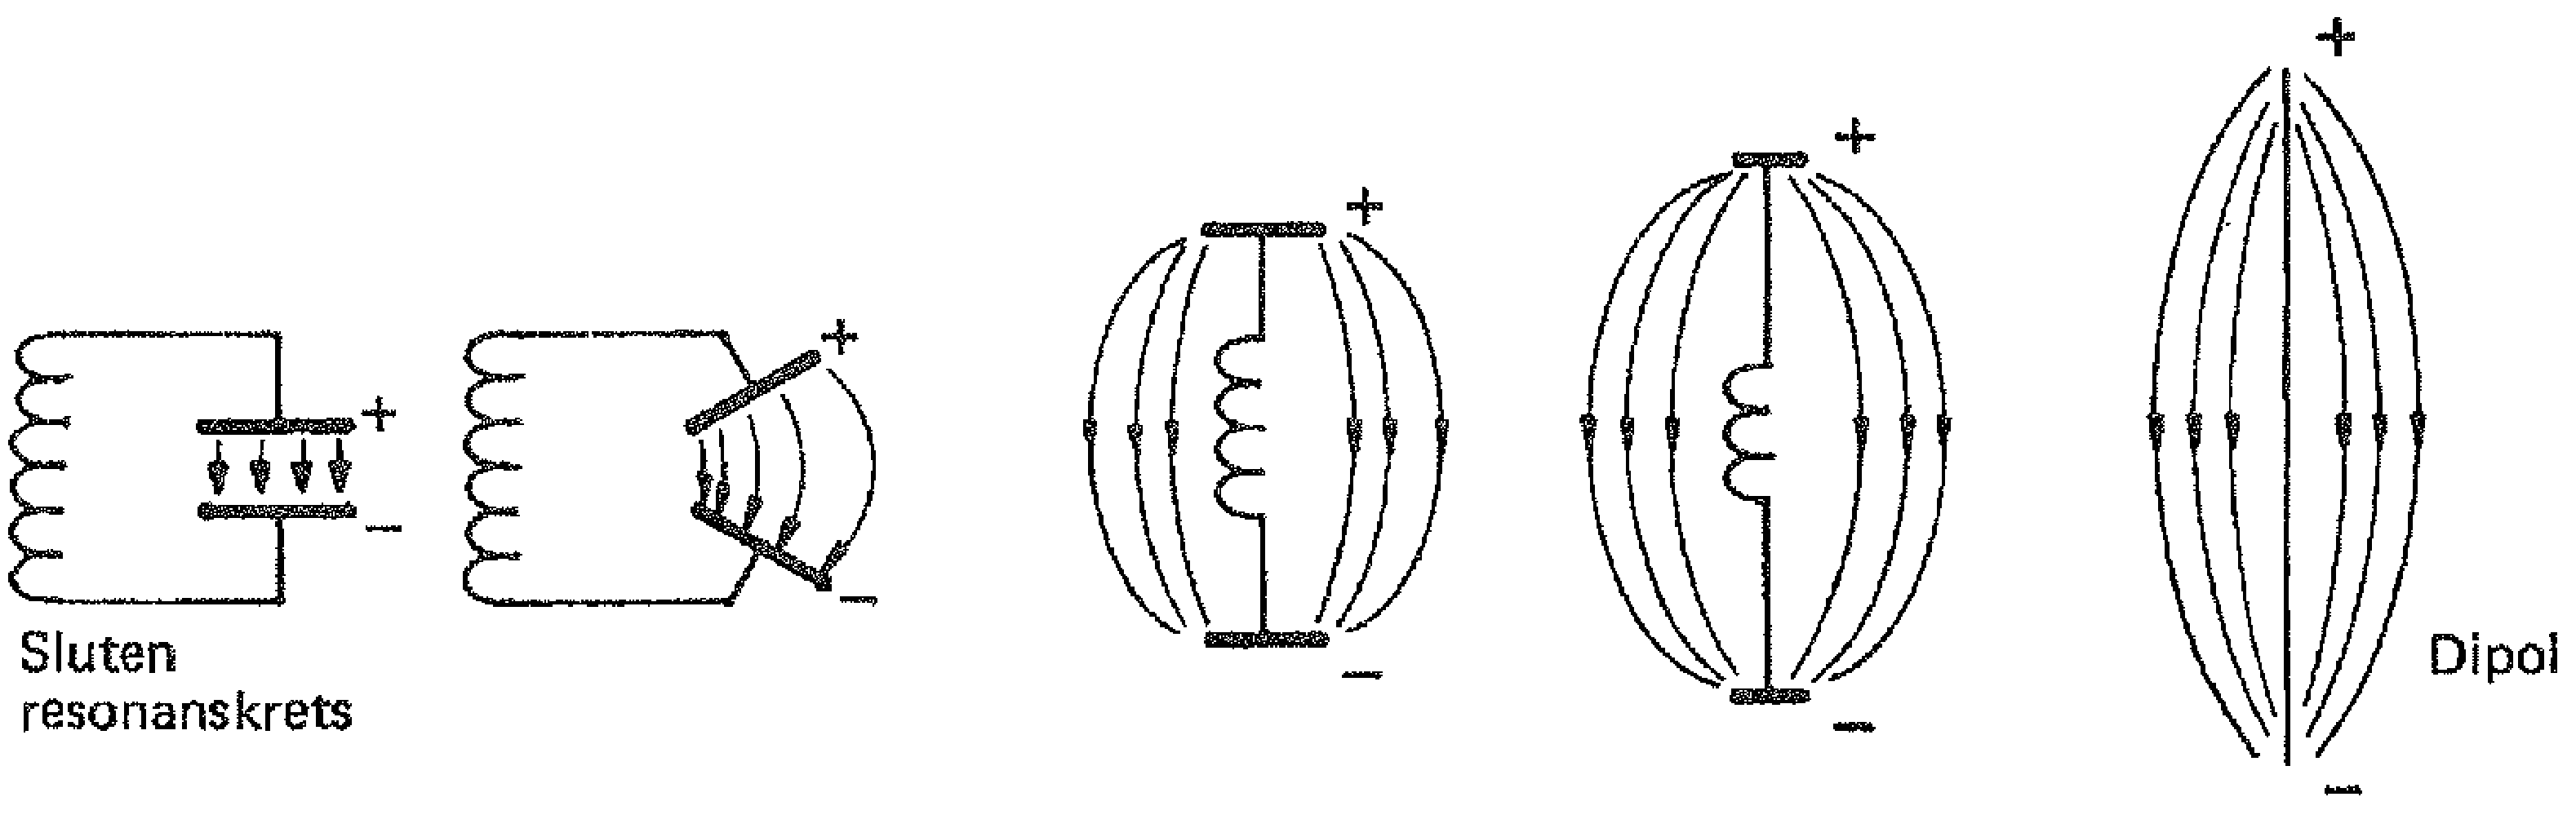
\includegraphics[width=\textwidth]{images/cropped_pdfs/bild_2_7-01.pdf}
\caption{Från sluten LC-krets till antenn}
\label{fig:BildII7-01}
\end{figure}

Vissa likheter finns mellan en mekanisk pendel och en elektriskt
svängningskrets.

\subsubsection{Mekanisk pendel}

Energin i en mekanisk pendel växlar mellan två
ytterlighetstillstånd. Det ena är när pendeln just vänder i ett
ytterläge. Då innehåller den mest lägesenergi och ingen
rörelseenergi. När pendeln rör sig mot mittläget, så omvandlas
lägesenergin till rörelseenergi. I mittläget, som är det andra
ytterlighetstillståndet, innehåller pendeln mest rörelseenergi och
ingen lägesenergi etc.

\subsubsection{Elektrisk svängningskrets}

Den elektriska svängningskretsen kan sägas motsvara den mekaniska
pendeln i den meningen att det i båda fallen pågår en ständig pendling
mellan lägesenergi och rörelseenergi. Se bild \ref{fig:BildII7-02}.

När strömmen i den elektriska svängningskretsen just upphört för att
vända, så innehåller kondensatorn mestladdning, d.v.s. det starkaste
elektriska fältet mellan elektroderna. Detta fält är lägesenergi. Den
utjämningsström som följer, från den ena elektroden över till den
andra, omges av ett magnetiskt fält. Detta fält är rörelseenergi.

Förloppet visas i bild \ref{fig:BildII7-02}, där det framgår att dipolen omges av
det starkaste elektriska fältet vid tidpunkten \(t=0\) samt vid
\(t=1/2T\) med omvänd polaritet, där T är periodtiden. Vidare att
dipolen omges av det starkaste magnetiska fältet vid tidpunkten
\(t=1/4T\) samt vid \(t=3/4T\) med omvänd strömriktning och
fältpolaritet.

\begin{figure}
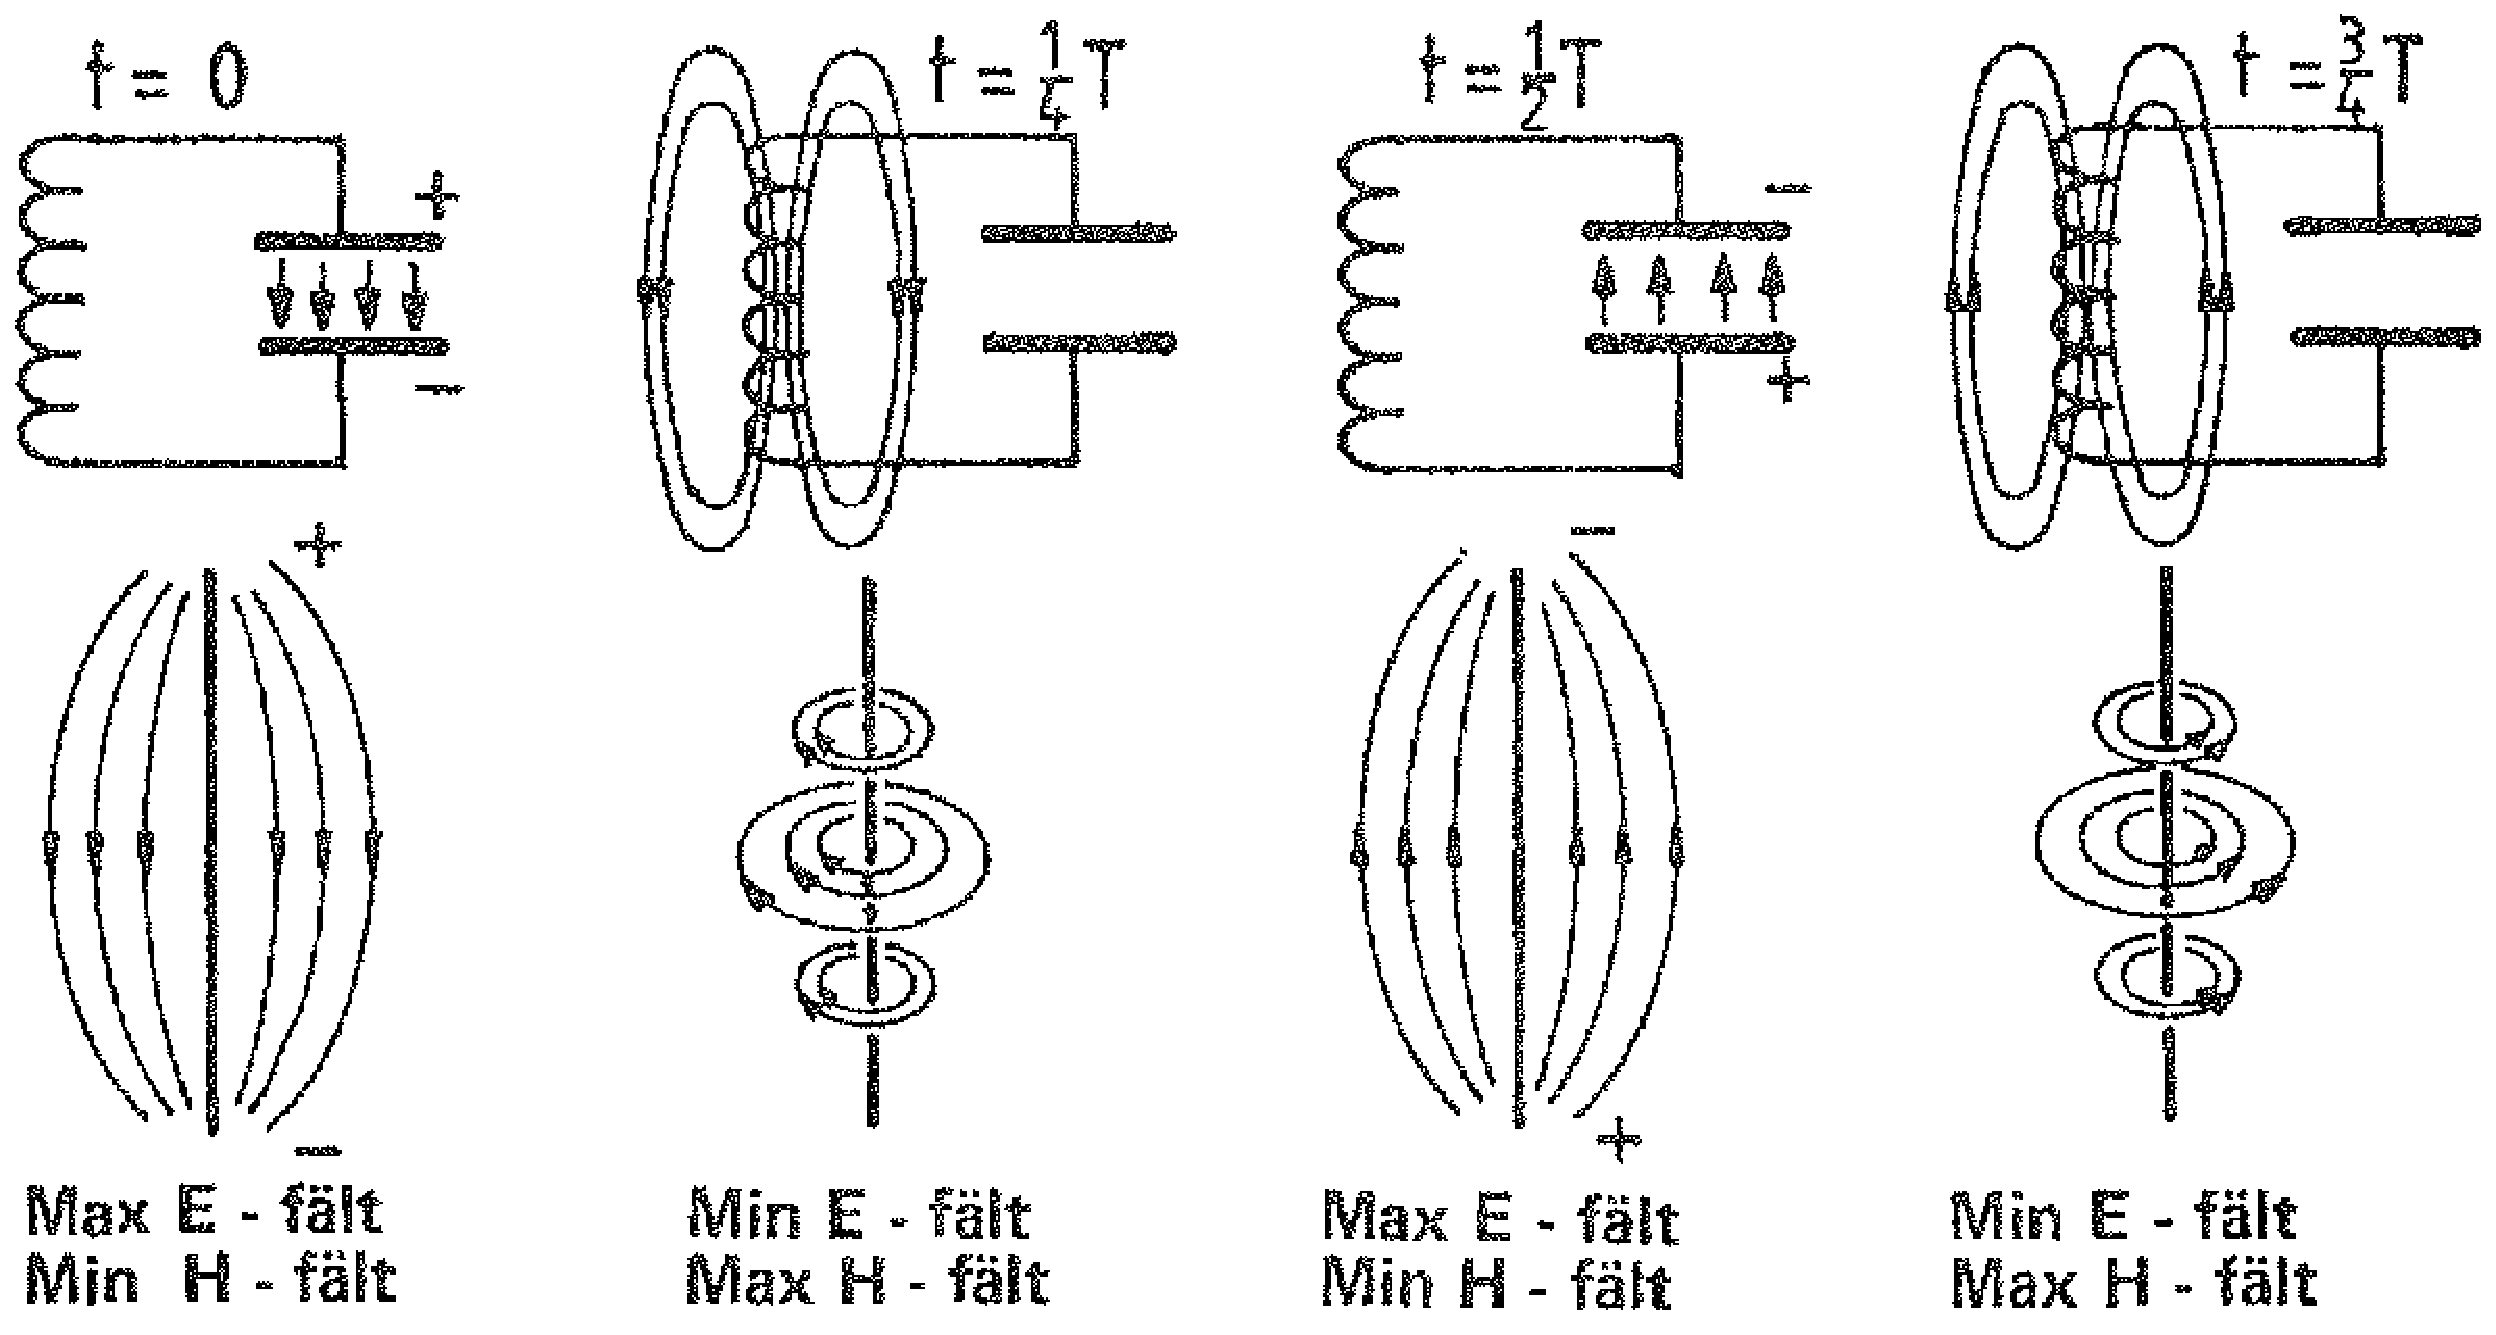
\includegraphics[width=\textwidth]{images/cropped_pdfs/bild_2_7-02.pdf}
\caption{Pendlingen mellan E-fält och H-fält}
\label{fig:BildII7-02}
\end{figure}

\begin{wrapfigure}{R}{0.5\textwidth}
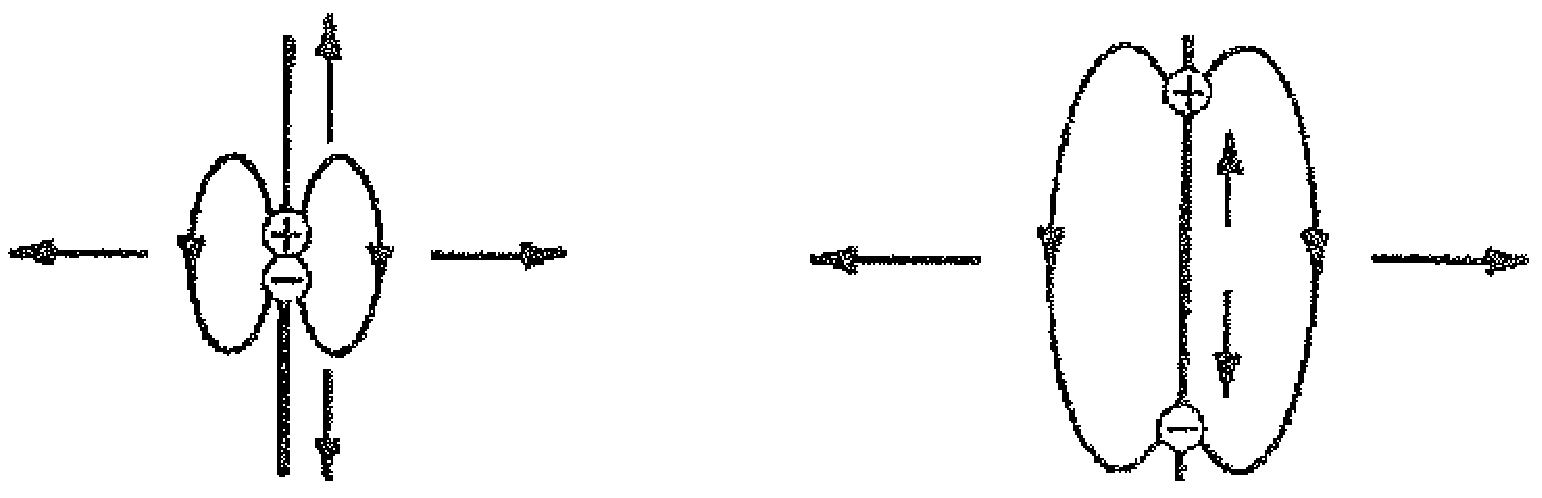
\includegraphics[width=0.5\textwidth]{images/cropped_pdfs/bild_2_7-03.pdf}
\caption{Elementär dipol}
\label{fig:BildII7-03}
\end{wrapfigure}

Med förklaringen av E- och H-fälten som bakgrund följer nu en enkel
framställning av hur radiovågor uppstår ur dessa fält.

Maxwell påvisade i sina ekvationer bl.a. sambandet mellan elektroner
i rörelse i en ledare och elektromagnetiska vågor i rummet. Vidare,
att elektroner som rör sig med avtagande eller tilltagande hastighet
avger elektromagnetisk energi.

Hur energi strålar från en ledare kan förklaras med en (tänkt)
elementär dipol, som genomflyts av växelström (Bild \ref{fig:BildII7-03}).

Dipolen består av två lika stora elektriska laddningar med motsatt
polaritet. När len matas med en växelström, så rör sig laddningarna
ständigt, omväxlande emot respektive ifrån varandra. Tänk på två kulor
i var sin ände av en spiralfjäder. Avståndet mellan laddningarna
ändras i takt med styrkan och riktningen på strömmen. Systemet är
alltså under ständig hastighetsändring (ökning resp. minskning),
vilket är förutsättningen för att energi ska strålas ut.

Först är laddningarna nära varandra på grund av liten laddning. Vid
ökande ström ökar avståndet mellan laddningarna och det byggs upp ett
mer utbrett och energirikt E-fält. Samtidigt byggs även ett H-fält upp
omkring dipolen, vinkelrätt mot E-fältet o.s.v. Detta gäller både för
en elementär dipol och en elektrisk ledare med många fria elektroner
(verklig antenn).

Formeln för det resulterande S-fältet är \(\overline{S} =
\overline{S}\cdot\overline{H}\), vilket visar att den lagrade energin
i dipolens närmaste omgivning ökar när avståndet (potentialen) mellan
dipolens laddningar ökar.

Bild \ref{fig:BildII7-04} visar hur ett E-fält byggs upp omkring en dipol och
avskiljs från den. De visade kraftlinjerna är E- fältet. H-fältet
visas inte, men ligger vinkelrätt mot E-fältet, i cirklar omkring
antennen. Se bild \ref{fig:BildII7-05}.

\begin{figure}
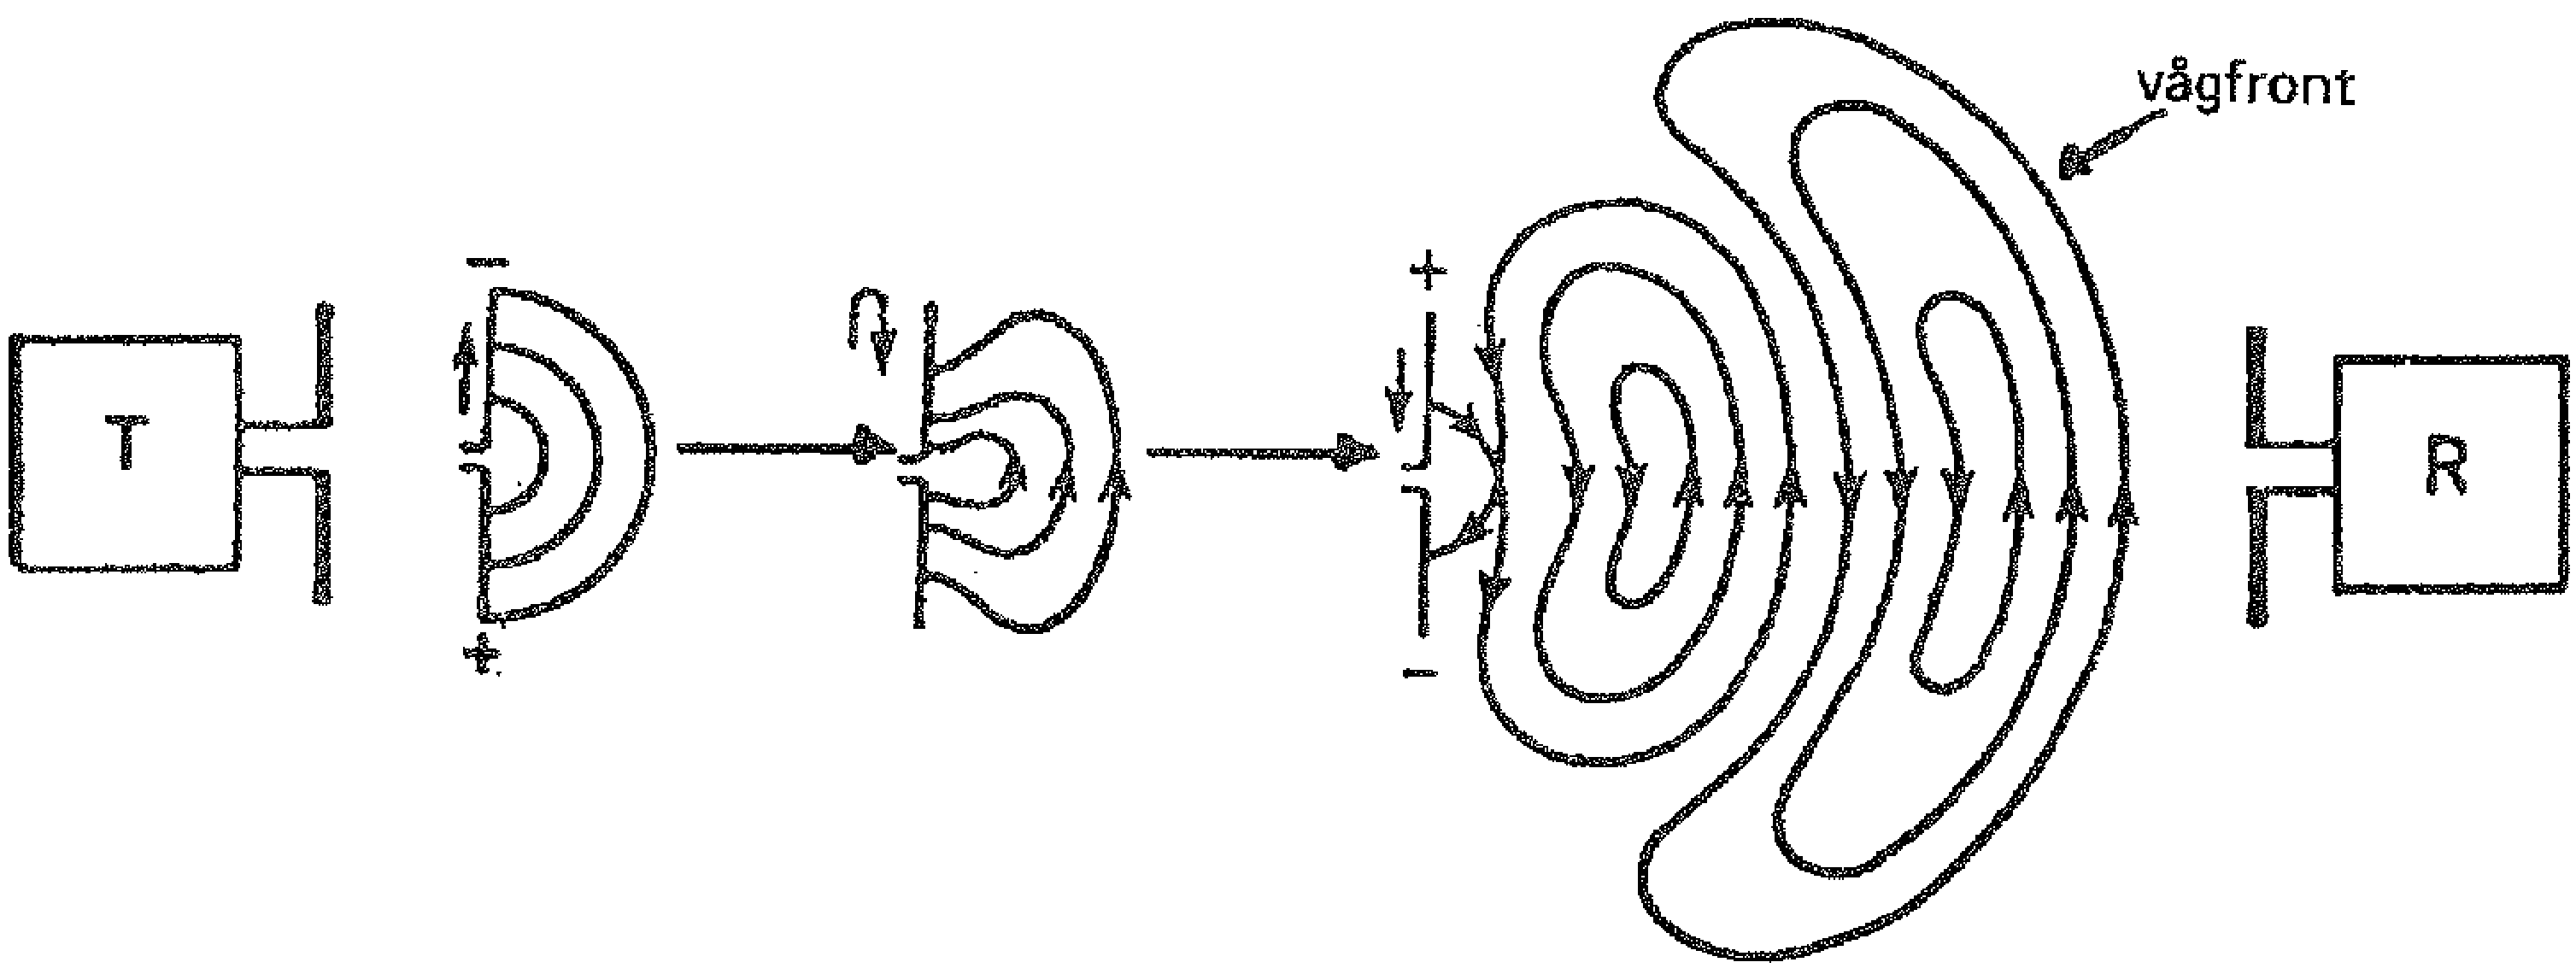
\includegraphics[width=\textwidth]{images/cropped_pdfs/bild_2_7-04.pdf}
\caption{Ett självständigt E-fält skapas}
\label{fig:BildII7-04}
\end{figure}

\begin{figure}
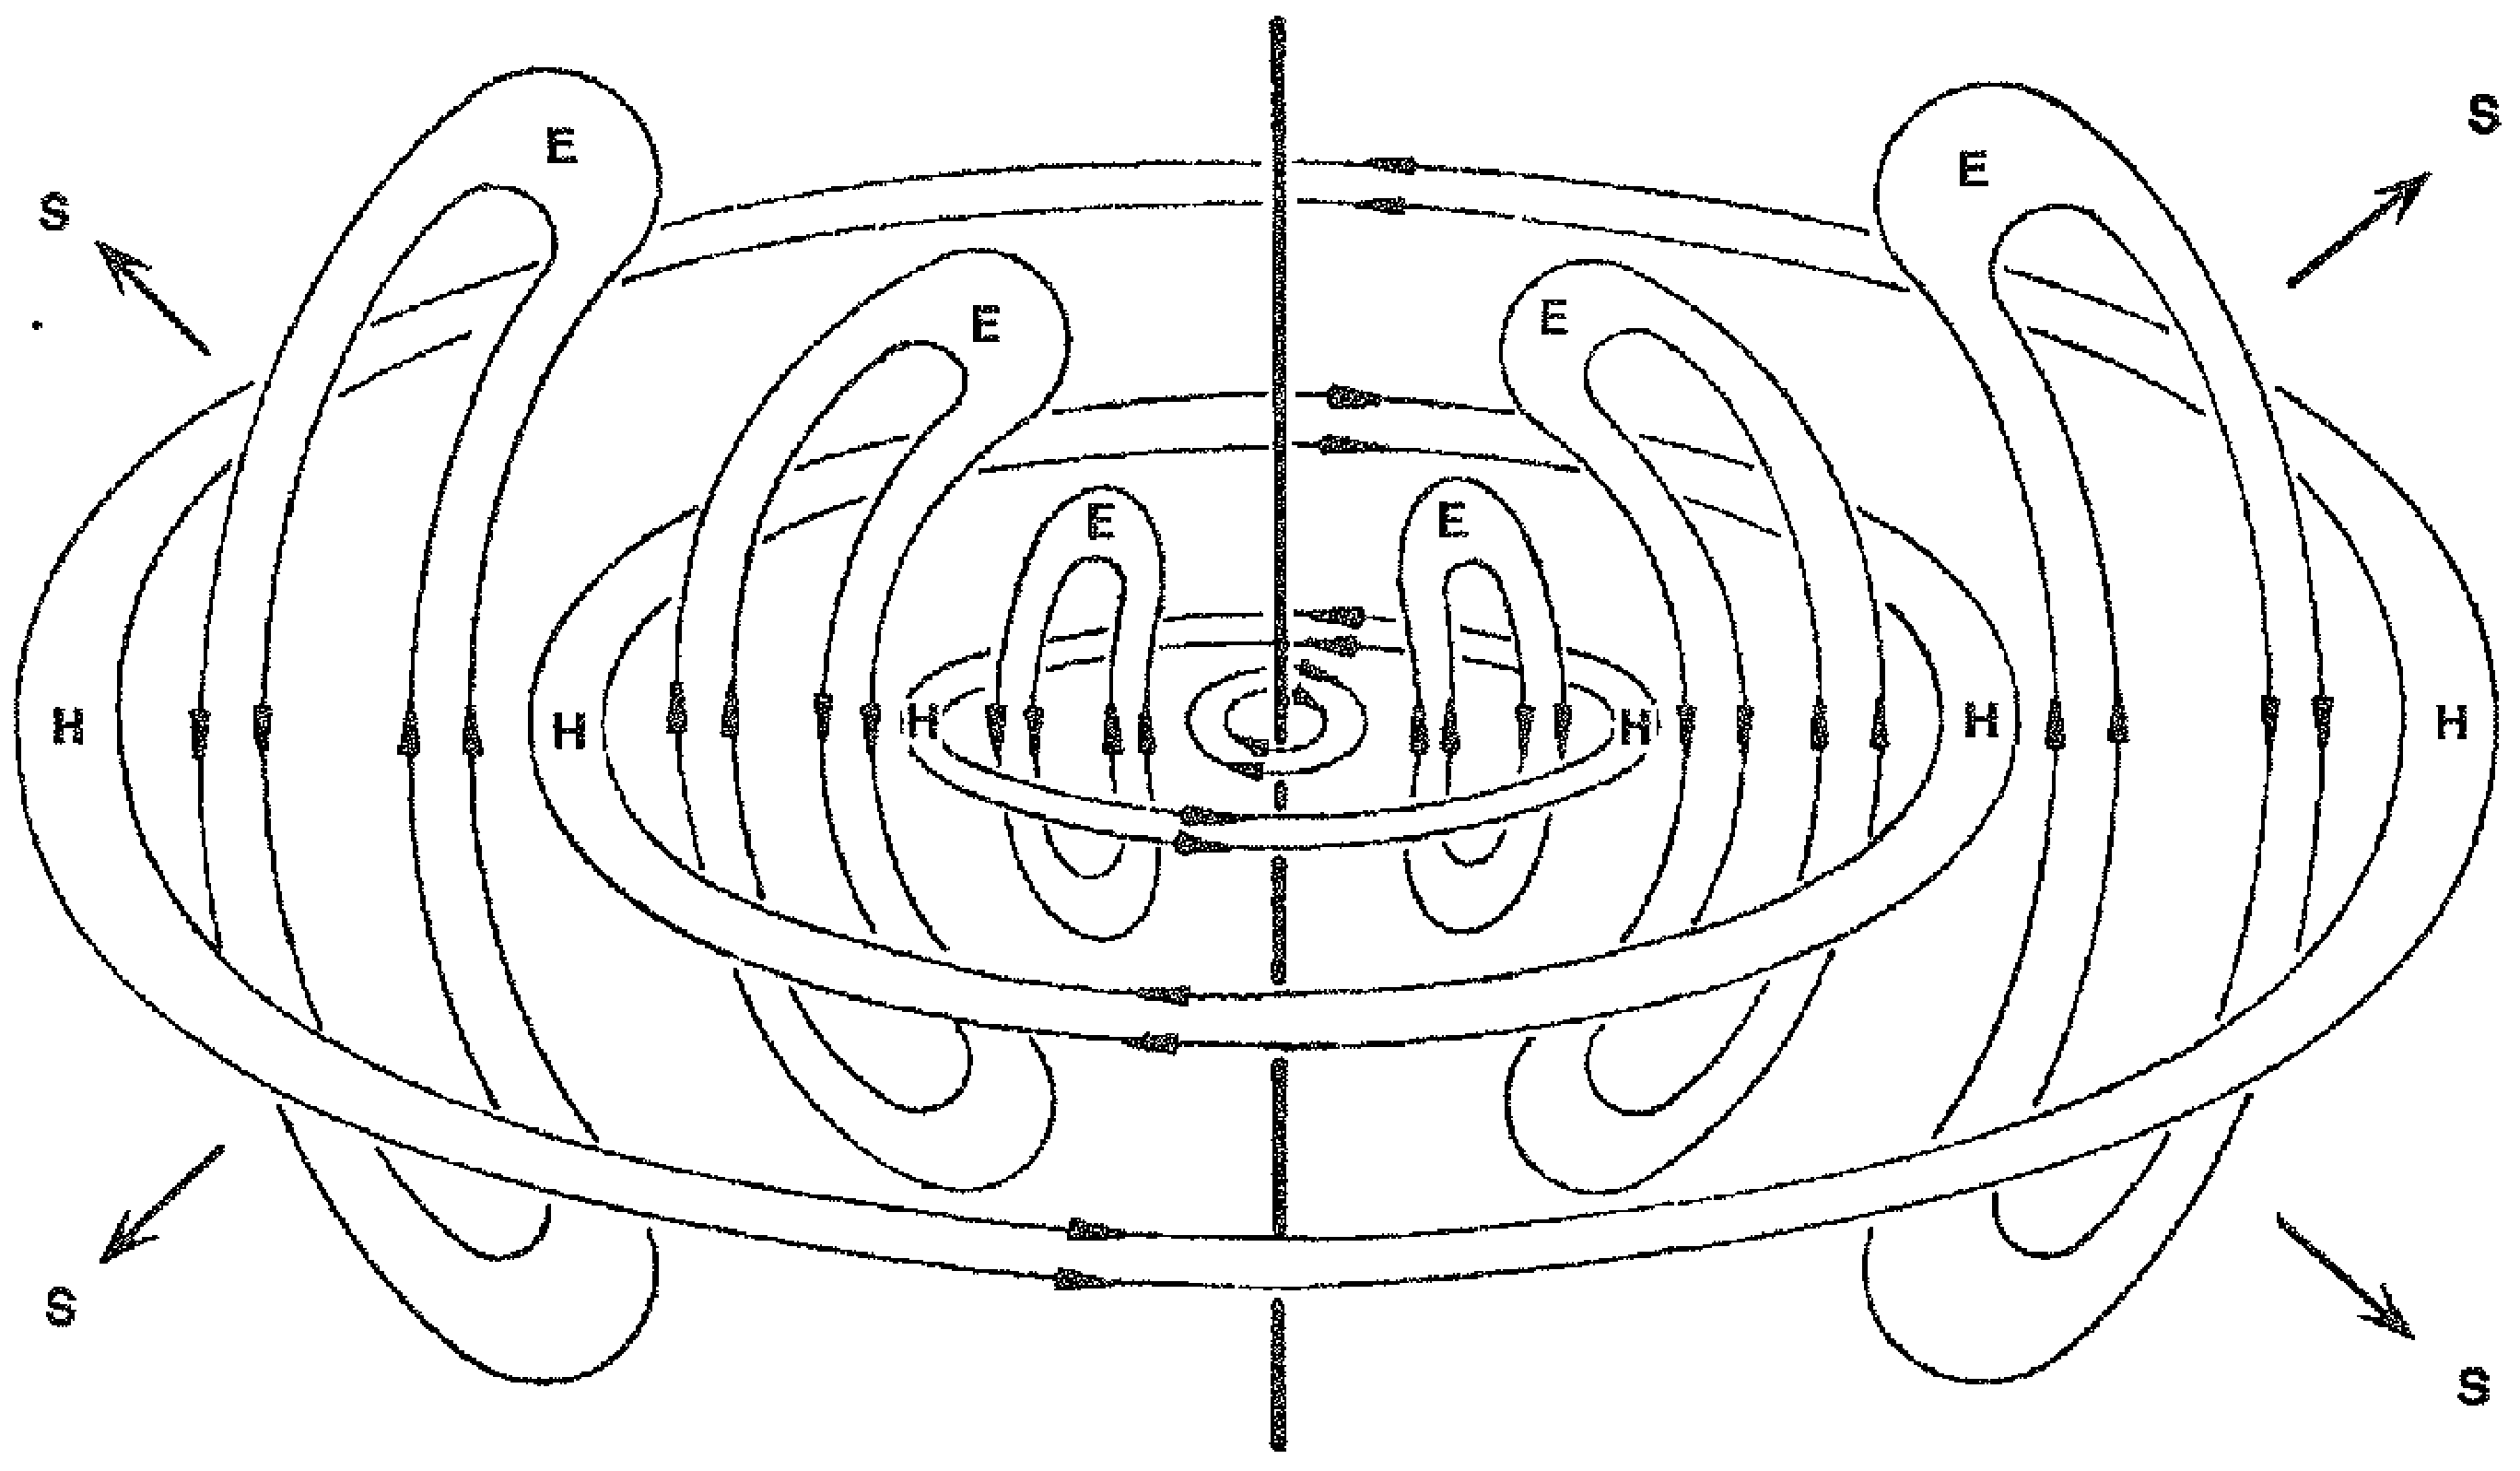
\includegraphics[width=\textwidth]{images/cropped_pdfs/bild_2_7-05.pdf}
\caption{E-, H- och B-fälten omkring en antenn (förenklad framställning)}
\label{fig:BildII7-05}
\end{figure}

När dipolens laddningar ändrar riktning och åter börjar att röra sig
emot varandra, börjar det E-fält som byggts upp att också byta
riktning. Men det kommer inte att falla tillbaka till dipolens mitt
utan sluts till ett eget kretslopp -- Maxwells första ekvation.
Jämför med en såpbubbla som lämnat blåsröret.
Omkring dipolen har det nu bildats ett självständigt E-fält, som sin tur
alstrar ett eget H-fält.

En period av en elektromagnetisk våg (ett S-fält) har alstrats och
fortsätter att utvidga sig. För varje följande period alstras ett nytt E-fält,
som separeras från antennen och bildar ett H-fält o.s.v.
Varje gång bildas alltså en ny ''fältbubbla'' inne i den föregående, vilken
håller på att utvidgas.

Resultatet är ett elektromagnetiskt fält, d.v.s. en radiovåg.

Som nämts består en radiovåg av ett högfrekvent elektromagnetiskt fält
(S). Det är i sin tur sammansatt av två andra fält, det elektriska E-
och det magnetiska H-fältet.  Energin i S-fältet fördelas lika mellan
E-fältet och H-fälten, vars krafter korsar varandra
vinkelrätt. S-fältet ligger i plan med både E- och H-fälten och breder
ut sig vinkelrätt mot dem. S-fältets riktning beror av den inbördes
riktningen på E- och H-fälten.

När E-fältet är vertikalt, sägs vågen vara vertikalt polariserad. När
samma fält är horisontellt sägs vågen vara horisontellt
polariserad. När E-fältet roterar i vågfrontens plan, och därmed även
H-fältet, sägs vågen vara cirkulärt polariserad.

Fälten framställs i text och bild som s.k. kraftlinjer med pilar som
föreställer kraftriktningen.
Linjernas längd föreställer fältets styrka.
Bild \ref{fig:BildII7-06} visar ett avsnitt av en vågfront S med vertikal
polarisation.

\begin{wrapfigure}{R}{0.5\textwidth}
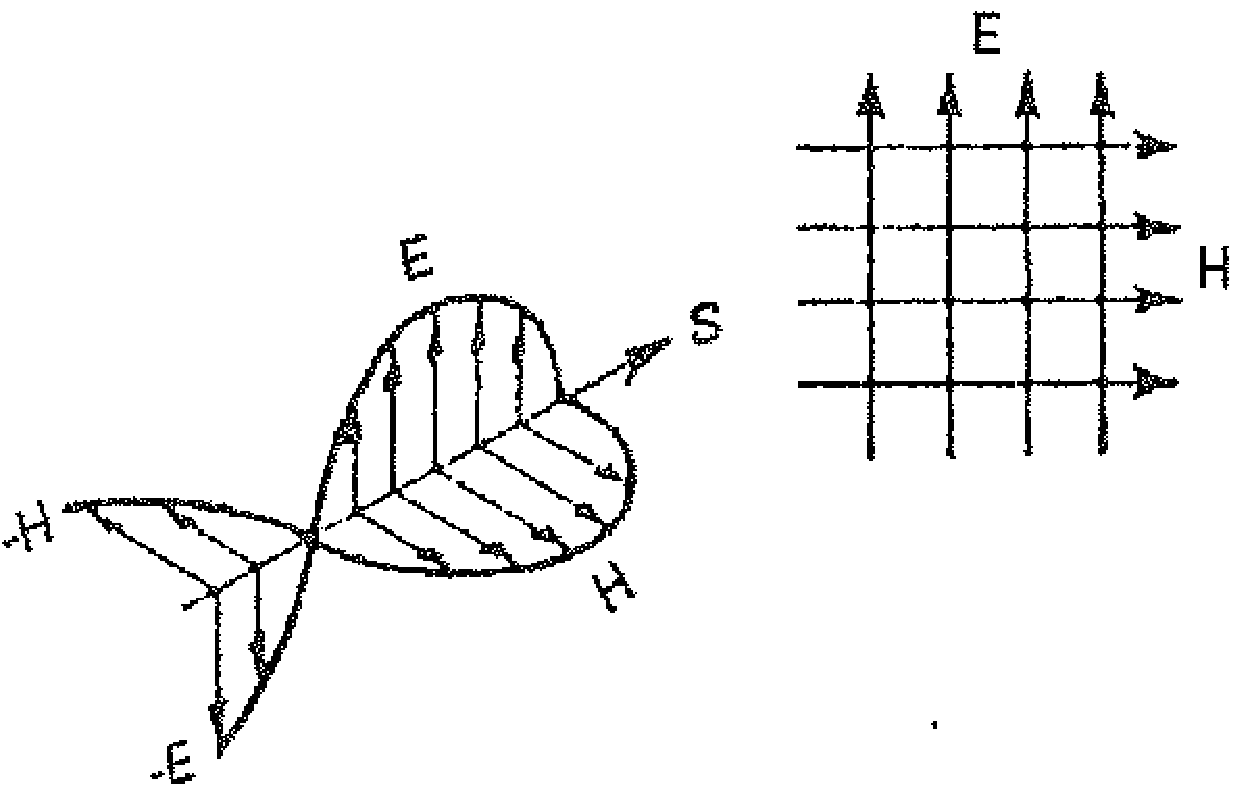
\includegraphics[width=0.5\textwidth]{images/cropped_pdfs/bild_2_7-06.pdf}
\caption{E-, H- och S-fält}
\label{fig:BildII7-06}
\end{wrapfigure}
